\question{1}{
    Defensie onderzoekt de stressbestendigheid van vrouwelijke en mannelijke militairen in potentieel levensbedreigende situaties.
    Tijdens een realistische simulatie van een hinderlaag in vijandelijk gebied wordt de hartslag gemeten van negen vrouwelijke en negen mannelijke militairen.
    De gemiddelde hartslag tijdens het 10 minuten durende scenario wordt per militair vastgelegd.
    
    De resultaten zijn als volgt:

    \begin{center}
        \begin{tabular}{c|ccccccccc}
            \toprule
                \textbf{Gemiddelde hartslag (vrouwen, $A$)} & $102$ & $110$ & $98$ & $120$ & $115$ & $105$ & $108$ & $112$ & $117$ \\
                \textbf{Gemiddelde hartslag (mannen, $B$)} & $108$ & $122$ & $130$ & $115$ & $125$ & $110$ & $118$ & $127$ & $121$ \\
            \bottomrule
        \end{tabular}
    \end{center}

    Het hoofd van de medische dienst wil weten of mannelijke militairen in deze setting een hogere stressrespons vertonen dan hun mannelijke collega's. 
    Voor beide populaties wordt aangenomen dat de gemiddelde hartslag normaal verdeeld is met onbekende verwachtingswaardes $\mu_A$ en $\mu_B$, en standaardafwijkingen $\sigma_A$ en $\sigma_B$.
}
    \begin{enumerate}[label=(\alph*)]
        \item Bereken de steekproefgemiddeldes $\overline{x_A}$ en $\overline{x_B}$, en de steekproefvarianties $s_A^2$ en $s_B^2$.
        \answer{
            {\bfseries Populatie $A$: vrouwelijke militairen.}
            We berekenen het steekproefgemiddelde $\overline{x_A}$ als volgt:
            \begin{align*}
                \overline{x_A} = \frac{ 102 + 110 + \ldots + 117 }{ 9 } \approx 109,6667.
            \end{align*}
        

            We berekenen de steekproefvariantie $s_A^2$ als volgt:
            \begin{align*}
                s_A^2 &= \frac{ (x_1 - \overline{x_A})^2 + (x_2 - \overline{x_A})^2 + \ldots + (x_n - \overline{x_A})^2 }{ n - 1 } \\
                &= \frac{ (102 - 109,6667)^2 + (110 - 109,6667)^2 + \ldots + (117 - 109,6667)^2 }{ 9 - 1 } \\
                &\approx 51,75.
            \end{align*}         
       
            {\bfseries Populatie $B$: mannelijke militairen.}

            We berekenen het steekproefgemiddelde $\overline{x_B}$ als volgt:
            \begin{align*}
                \overline{x_B} = \frac{ 108 + 122 + \ldots + 121 }{ 9 } \approx 119,5556.
            \end{align*}
        

            We berekenen de steekproefvariantie $s_B^2$ als volgt:
            \begin{align*}
                s_B^2 &= \frac{ (y_1 - \overline{x_B})^2 + (y_2 - \overline{x_B})^2 + \ldots + (y_n - \overline{x_B})^2 }{ m - 1 } \\
                &= \frac{ (108 - 119,5556)^2 + (122 - 119,5556)^2 + \ldots + (121 - 119,5556)^2 }{ 9 - 1 } \\
                &\approx 56,2778.
            \end{align*}        
        }

        \item Bepaal met behulp van een $F$-toets of de varianties in de gemiddelde hartslag gelijk zijn voor de populaties van vrouwelijke en mannelijke militairen.
            Gebruik de $p$-waarde in je conclusie. 
            Kies voor het significantieniveau $\alpha = 0,05$.
        \answer{
            We noteren de populaties vrouwelijke en mannelijke militairen respectievelijk met $A$ en $B$.
            In de vraag staat dat we aan mogen nemen dat $X_A \sim N(\mu_A=?; \sigma_A=?)$ en $X_B \sim N(\mu_B=?; \sigma_A=?)$.

            We toetsen op gelijke varianties, oftewel de nulhypothese $H_0$ en de alternatieve hypothese $H_1$ worden als volgt gedefinieerd:
            \begin{align*}
                H_0: \quad \sigma_A^2 = \sigma_B^2 \\
                H_1: \quad \sigma_A^2 \neq \sigma_B^2
            \end{align*}

            Verder is gegeven dat we mogen werken met een significantieniveau $\alpha=0,05$, en data is al verzameld voor beide populaties.
            De toetsingsgrootheid voor een $F$-toets is gelijk aan
            \[
                F = \frac{S_A^2}{S_B^2}, 
            \]
            en volgt een $F(n-1, m-1)$-verdeling, oftewel een $F(8, 8)$-verdeling.

            De geobserveerde toetsingsgrootheid is gelijk aan
            \[
                f = \frac{s_A^2}{s_B^2} = \frac{51,75}{56,2778} \approx 0,9195.
            \]
            
            In dit geval is de $p$-waarde gelijk aan de linkeroverschrijdingskans van deze toetsingsgrootheid $f$ (deze is kleiner dan de linkeroverschrijdingskans):
            \begin{align*}
                p = P(F \le f) = \text{Fcdf}(\text{lower}=0; \text{upper}=0,9195; \text{df1}=9; \text{df2}=9) \approx 0,4542.
            \end{align*}
            Aangezien de $p$-waarde groter is dan $\alpha/2 = 0,025$ (tweezijdige toets!), wordt de nulhypothese $H_0$ aangenomen.
            Er is onvoldoende bewijs om op basis van deze steekproef de aanname van gelijke varianties te verwerpen.
            We mogen dus uitgaan van gelijke varianties.

            \begin{center}
                \resizebox{0.9\textwidth}{!}{
                    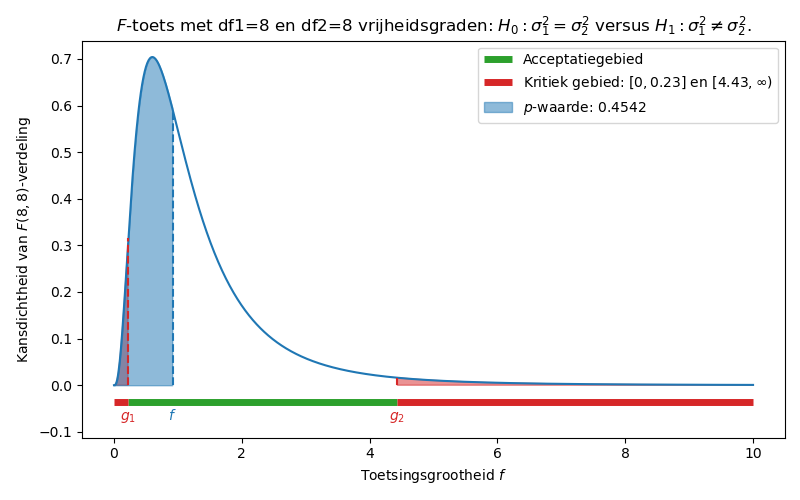
\includegraphics{oefenopgave1_Ftoets.png}
                }
            \end{center}
        }

        \item Bepaal met behulp van een onafhankelijke $t$-toets of de gemiddelde hartslag in stresssituaties bij mannelijke militairen significant hoger ligt dan bij vrouwelijke militairen.
            Baseer je conclusie op het kritieke gebied.
            Kies opnieuw voor het significantieniveau $\alpha = 0,05$.
        \answer{
            We toetsen of de gemiddelde hartslag $\mu_B$ voor mannelijke militairen significant hoger is dan de gemiddelde hartslag $\mu_A$ voor vrouwelijke militairen.
            De hypotheses kunnen we daarom als volgt defini\"eren:
            \begin{align*}
                H_0: \quad \mu_A \ge \mu_B \text{ (niet significant hoger) } \\
                H_1: \quad \mu_A < \mu_B \text{ (wel significant hoger) }
            \end{align*}

            Verder is gegeven dat we mogen werken met een significantieniveau $\alpha=0,05$, en data is al verzameld voor beide populaties.

            Op basis van ons antwoord bij vraag (b) mogen we aannemen dat $\sigma = \sigma_A = \sigma_B$.
            Dat betekent dat we met de pooled variance mogen werken als schatting voor de gemeenschappelijke onbekende $\sigma$.
            
            \begin{align*}
                s_P^2 = \frac{(n-1)\cdot s_A^2 + (m-1) \cdot s_B^2}{n-1+m-1} = \frac{8 \cdot 51,75 + 8 \cdot 56,2778}{16} \approx 54,0139.
            \end{align*}
            
            De toetsingsgrootheid van de bijbehorende $t$-toets is (onder de nulhypothese $\mu_A = \mu_B$) gelijk aan
            \begin{align*}
                t &= \frac{(\overline{x_A}-\overline{x_B}) - (\mu_A - \mu_B)}{\sqrt{\frac{s_P^2}{n} + \frac{s_P^2}{m}}} \\
                  &= \frac{(109,6667 - 119,5556) - 0}{\sqrt{\frac{54,0139}{9} + \frac{54,0139}{9}}} \\
                  &\approx -2,8543, 
            \end{align*}

            en komt uit een $t$-verdeling met $\text{df}=n+m-2=16$ vrijheidsgraden.
            Omdat we linkszijdig toetsen, is het kritieke gebied van de vorm $(-\infty; g]$.
            Deze kritieke grens kunnen we met de $t$-verdeling bepalen, namelijk
            \[
                g = \invt(\text{opp} = \alpha; \text{df}=n+m-2) = \invt(\text{opp}=0,05; \text{df}=16) \approx -1,7459
            \]
            
            De toetsingsgrootheid $t$ ligt dus in het kritieke gebied, dus $H_0$ moet worden verworpen.
            Er is op basis van deze steekproeven voldoende reden om aan te nemen dat de gemiddelde hartslag van mannelijke militairen in stresssituaties significant hoger ligt dan bij vrouwelijke militairen.
            \begin{center}
                \resizebox{0.9\textwidth}{!}{
                    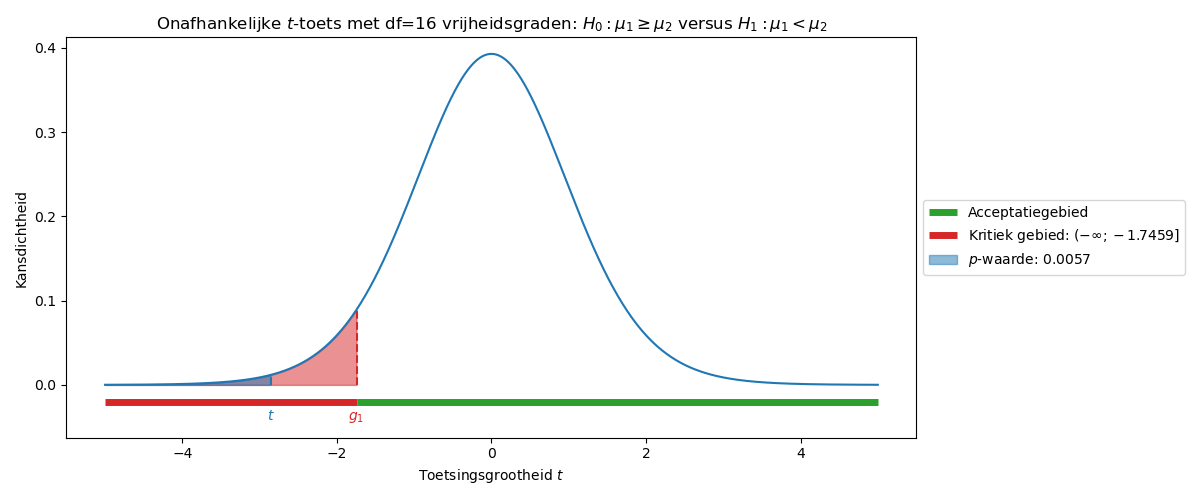
\includegraphics{oefenopgave1_ttoets.png}
                }
            \end{center}
        }    
    
    \end{enumerate}